\documentclass[10pt]{article}

%---------------------------------------------------------------------
\usepackage[a4paper, headsep=-4in,bindingoffset=0in,%
left=2.5cm,right=2.5cm,top=2.5cm,bottom=2.5cm,%
footskip=.25in]{geometry}

%\usepackage[english]{babel}   
\usepackage[utf8]{inputenc}  
\usepackage{tgbonum}
\usepackage[font=scriptsize]{caption}

%\DeclareCaptionFont{6pt}{\fontsize{6pt}{6pt}\selectfont}
\captionsetup[figure]{font={stretch=1}}  
%\usepackage{sectsty}
\usepackage{subcaption}
\usepackage{wrapfig}
\usepackage{layout}
\usepackage{graphicx}
\usepackage{verbatim}
\usepackage{listings}
\usepackage{mathptmx}

\usepackage[backend=biber,style=apa,sorting=none]{biblatex}
\addbibresource{paperpile.bib}
%\pagenumbering{gobble}
\pagenumbering{arabic}

\usepackage{amsfonts}
\graphicspath{{figs/}}
\setlength{\topmargin}{-10pt}
%\renewcommand{\baselinestretch}{1.5}

\usepackage{indentfirst}
\setlength{\parindent}{1cm}

\setlength{\headsep}{1pt}
%---------------------------------------------------------------------

\begin{document} 

\begin{center}
{\large \section*{Systematic comparison of out-of-sample performance of imaging biomarkers of chronic stroke motor outcome }}
\end{center}

\begin{center}
Emily Olafson$^1*$, Keith Jamison$^1$, Amy Kuceyeski$^1$
\end{center}

    1. \textmd{Department of Radiology, Weill Cornell Medical College, New York City, New York, USA, 10021} 

%---------------------------------------------------------------------

\section{Abstract}
Ischemic stroke is a major cause of physical impairment, and up to a third of stroke survivors have poor motor outcomes five years after the event. However, the ability to predict long-term deficits from acute clinical information remains a challenge. The location of the stroke in the brain can explain some of the variance in long-term outcomes, and incorporating information about lesion location can improve prediction models. Automated lesion segmentation methods can now be used, but it is unclear how to optimally use volumetric lesion data to predict chronic motor outcomes. Several lesion biomarkers have been related to stroke motor outcome, but it is unclear whether they can accurately predict chronic impairments across a range of lesion topographies. Models that incorporate damage to additional sensorimotor regions beyond the primary motor cortex have been shown to explain more variance in post-stroke outcome than models that only incorporate primary motor cortex CST damage. These models typically incorporate damage to premotor, supplementary motor, pre-supplementary motor, and somatosensory cortices. Few studies have assessed the performance of these models with cross-validation. This paper presents a comparison of the predictive accuracy of several imaging biomarkers of post-stroke motor impairment using the ENIGMA dataset, a multi-site stroke lesion database. The models are compared using out-of-sample performance, and the results show that data-driven features outperform theory-driven features. The data-driven features also outperform models trained on chronic subjects when applied to acute subjects. These results highlight the potential of data-driven feature selection in identifying lesion-deficit associations beyond current theory-driven biomarkers.

\section{Introduction}
Ischemic stroke is a leading cause of physical impairment worldwide. Up to one-third of stroke survivors have poor motor outcomes five years after stroke, but the ability to predict long-term deficits from acute clinical information is still a major challenge.

The location of the stroke in the brain explains some of the variance in long-term outcomes, and prediction models of stroke outcome are improved by incorporating information about lesion location. Lesion segmentations, once requiring  delineation by experts, can now be performed with automated methods requiring minimal manual editing (\cite{Pustina2016-qu}). However, it is currently unclear how to optimally use volumetric lesion data to predict chronic motor outcomes (\cite{Sperber2020-kp, Kasties2021-rm}). 

Several lesion biomarkers have been related to stroke motor outcome. The most widely-employed lesion biomarker of motor outcome is the corticospinal tract (CST) lesion load, or the proportion of voxels in the ipsilesional corticospinal tract (typically fibers from primary motor cortex) that intersect with the lesion (\cite{Zhu2010-qh, Feng2015-du}). This biomarker has been related to motor deficits in the acute phase of stroke, but it is unclear whether this biomarker can accurately predict chronic impairments across a wide range of lesion topographies (for review, see \cite{Kim2017-xe}). Models that incorporate information about how the lesion damages additional sensorimotor regions, i.e. regions beyond the primary motor cortex that are still related to motor and sensory function, explain more variance in post-stroke outcome compared to models that incorporate information about primary motor cortex CST damage alone (\cite{Ito2022-em, Sperber2021-lw, Rondina2016-ds, Rondina2017-ij, Schulz2012-yy}). These more complex models tend to incorporate damage to premotor, supplementary motor, pre-supplementary motor, and somatosensory cortices (\cite{Ito2022-em,Schulz2012-yy, Sperber2021-lw, Rondina2016-ds, Rondina2017-ij}). 

These biomarkers have typically been associated with motor scores within a sample. Variables that significantly relate to outcomes and variables that are predictively relevant can agree or diverge (\cite{Bzdok2020-py}). The practical performance of a predictive model must be evaluated by its performance on external data; i.e., by standard cross-validation (\cite{Hastie2001-or}). Although lesion load has been consistently related to motor outcomes, few studies have assessed the performance of models with cross-validation (for review, see \cite{Kim2017-xe}).

Indeed, the optimal set of features extracted from lesion data may not be directly related to hemiparesis per se (\cite{Bzdok2020-py, Sperber2021-lw}). Because of the hierarchical, non-random distribution of lesion topography (\cite{Mah2014-cb,Wang2019-dz}), damage to voxels outside of the motor system may meaningfully predict chronic motor impairment (\cite{Sperber2021-lw}). Machine learning models that incorporate features in a data-driven way may be able to discover lesion-deficit associations beyond the current suite of theory-driven biomarkers like those in the motor system (\cite{Kasties2021-rm, Calesella2021-kp}). We generate a measure of structural disconnection for all cortical and subcortical areas of the brain using the Network Modification tool, and use data-driven feature selection to identify regions that are relevant for the prediction of motor outcomes. 


In this paper, we robustly compare the predictive accuracy of several imaging biomarkers of post-stroke motor impairment by assessing their out-of-sample performance using the ENIGMA dataset, a multi-site stroke lesion database (\cite{Liew2020-ps}). We compare theory-driven features (i.e. motor-related CST lesion load) with data-driven imaging features. 



\section{Methods}



\subsection{Model specification}
All code to calculate lesion load is available on GitHub. 

\subsubsection{Lesion load of primary motor cortex}
The M1-corticospinal tract segmentation was obtained from the sensorimotor area tract template (SMATT) (\cite{Archer2018-ti}). M1-CST lesion load was calculated as the proportion of lesioned voxels intersecting with the ipsilesional M1-CST (\cite{Zhu2010-qh}).

\subsubsection{Lesion load of all corticospinal tract bundles}

Previously, \cite{Ito2022-em} have shown that models that use the corticospinal tract lesion load fibers originating the ventral premotor cortex in addition to lesion load of the primary motor cortex have the strongest associations with motor scores.

Corticospinal tract segmentations were obtained from the sensorimotor area tract template (SMATT), a set of 6 tracts derived from probabilistic tractography seeded in primary motor cortex (M1), dorsal and ventral premotor cortex (PMd and PMv, respectively), supplementary motor area (SMA), pre-supplementary motor area (pre-SMA), and primary somatosensory cortex (S1) (Figure \ref{fig1}) (\cite{Archer2018-ti}). Lesion load for each tract was calculated as:
\begin{equation}
    \textit{Lesion load} = \frac{\textit{Number of lesioned voxels that intersect with the tract}}{\textit{Sum of voxels in tract}}
\end{equation}

Motor scores were predicted using ridge regression models with ipsilesional lesion load (6 values) and bihemispheric lesion load (12 values, preserving left/right) as inputs. Lesion load values were normalized (subtracting the mean and dividing by the l2-norm) prior to model fitting. CST from all bundles were positively correlated with one another and negatively correlated with motor scores (Figure \ref{smatt_pairwise_correlations})

\subsubsection{Data-driven feature selection}
%\subsubsection*{Deriving ChaCo scores (change in connectivity) from lesion masks}

\begin{figure}[htp]
\centering
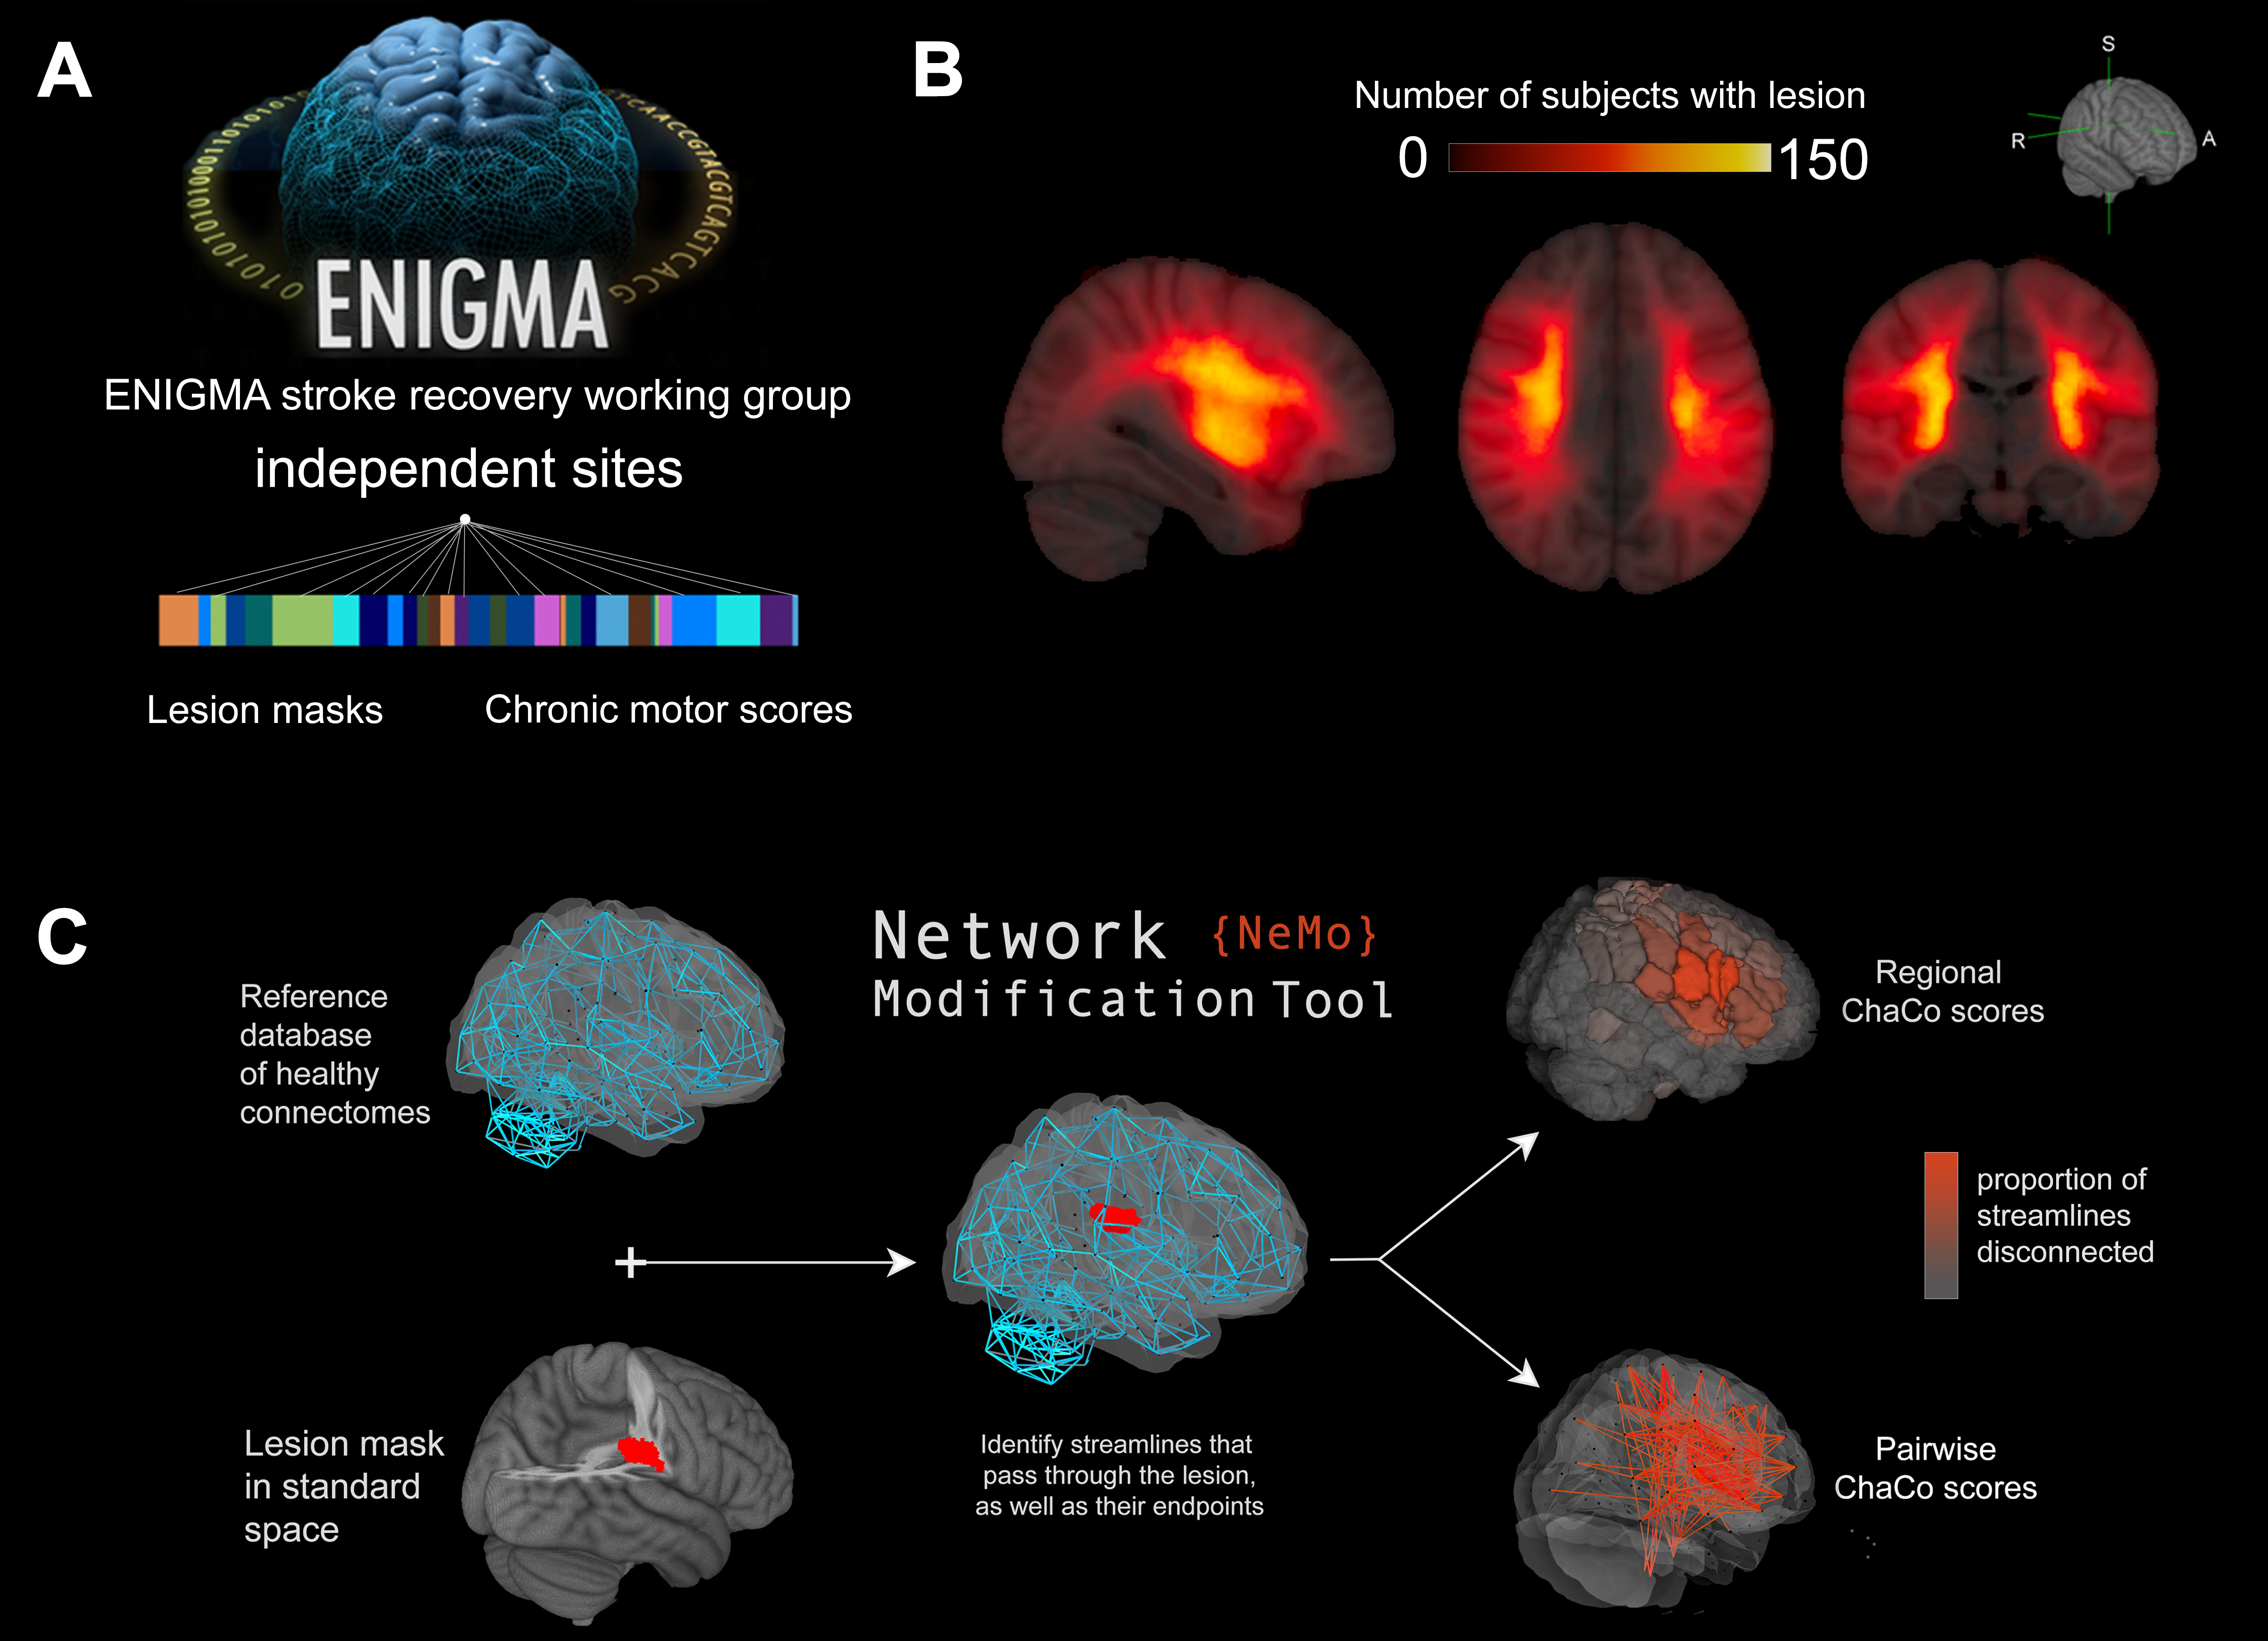
\includegraphics[width=1.0\linewidth]{figures/Multi-panelML.png}
\caption{Overview of the Network Modification tool. Binary lesion masks in MNI space representing the presence of a stroke lesion in a given voxel are provided by the user. Each lesion mask is embedded into 420 unrelated healthy structural connectomes (separately for each healthy subject) and the regional or pairwise change in connectivity (ChaCo) scores are calculated and averaged across healthy subjects. }
\label{fig1}
\end{figure}
Lesion masks in $1mm^3$ MNI v6 space were processed with the Network Modification Tool v2 (NeMo) pipeline (\cite{Kuceyeski2013-nk}) (https://github.com/kjamison/nemo for more detailed information). Given a lesion mask, the NeMo tool produces outputs that reflect the impact of the lesion on the white matter tracts connecting brain regions. The NeMo tool identifies every white matter streamline that intersects with a lesion and determines the brain regions at the endpoints of those streamlines, whose structural connections we expect to be disrupted (Figure \ref{nemotool}). The NeMo tool uses a reference structural connectome (SC) dataset of 420 unrelated subjects from the Human Connectome Project Young Adult database. Structural connectivity for HCP subjects was obtained using deterministic tractography (SD stream) with dynamic seeding, with additional SIFT2 weighting for each of 5 million streamlines (\cite{Smith2015-eb}).


We extracted two outputs from the NeMo tool that reflect the impact of the lesion on connectivity between brain regions:

\begin{enumerate}
\item Regional change in connectivity (ChaCo) scores: the ratio of (disrupted streamlines)/(total streamlines) for each region.
\item Pairwise change in connectivity (ChaCo) score: the ratio of (disrupted streamlines)/(total streamlines) for each region-pair.
\end{enumerate}

We employed ridge regression to account for multicollinearity of selected features. Ridge regression models were trained and evaluated using a 5-fold nested cross-validation loop. In the outer loop, the data was split into training and test partitions. Training data was further partitioned into training and validation in the inner loop. In the inner loop, two hyperparameters were optimized: the amount of regularization on regression coefficients ($\lambda$) and the number of features to include ($\kappa$) after a feature selection step. 
Because inference and prediction are different goals and the feature maps derived from both types of studies can vary widely (\cite{Sperber2021-lw, Bzdok2020-py}), we included a correlation-based feature selection step. 
The correlation between all features and the outcome was calculated and the features were ranked by absolute value correlation. The top $\kappa$ features were then included in the model, where $\kappa$ is chosen via nested cross-validation. Importantly, this feature selection was performed after data was split into training and test sets, such that no hold-out test data is used in the selection of the set of feature weights (\cite{Hastie2001-or}). 
 
 
The $\kappa$ values searched for FS86 spanned 30 values from 5 to 86, in log base-2 steps; the $\kappa$ values searched for shen268 spanned 30 values from 5 to 268, in log base-2 steps. The regularization coefficient $\lambda$ was chosen via grid search between $\lambda = 10^{-2}$ and $10^2$ in base-10 logarithmic steps for FS86, and between $\lambda = 10^{-2}$ and $10^3$ in base-10 logarithmic steps for Shen-268. 

\subsubsection{Ensemble models}
We evaluated whether performance would be improved by averaging predictions from the lesion load models and from the data-driven feature selection ChaCo models. These ensemble models were generated by running ChaCo-models and lesion load models separately, on the same subjects and with the same training/test/validation splits, and averaging the final predicted scores for each subject. The model performance was calculated using the averaged prediction scores.

\subsubsection{Model performance}
The performance of the model was assessed by calculating the coefficient of determination ($explained\_variance\_score$ in sklearn), or $R^2$, which captures the percent of variation in cognitive scores explained by the variation in the model predictors:
\begin{equation}
    R^2(y, \hat{y}) = 1 - \frac{Var(y-\hat{y})}{Var(y)}
\end{equation}
and by Pearson's correlation coefficient, 
\begin{equation}
    r(y, \hat{y}) = \sqrt{\frac{\sum_i{\hat{y}-\bar{y}}}{\sum_i{y-\bar{y}}}}
\end{equation}

\begin{tabular}{|l|l|r|r|r|r|}
%\captionof{table}{Site-specific demographic data.}
\hline {} &  Site &   N. &  N. F &  Mean age &  Mean normed motor \\ \hline
\textbf{0 } &  r001 &  39 &         10 &     59.62 &               0.62 \\ 
\textbf{1 } &  r002 &  12 &          6 &     65.75 &               0.45 \\
\textbf{2 } &  r003 &  15 &          6 &     59.53 &               0.26 \\ 
\textbf{3 } &  r004 &  19 &          7 &     44.63 &               0.20 \\ 
\textbf{4 } &  r005 &  27 &         12 &     64.93 &               0.67 \\
\textbf{5 } &  r009 &  57 &         16 &     67.84 &               0.92 \\ 
\textbf{6 } &  r010 &  26 &          7 &     57.15 &               0.97 \\ 
\textbf{7 } &  r011 &  28 &         10 &     57.21 &               0.89 \\ 
\textbf{8 } &  r015 &  15 &          0 &     59.60 &               0.72 \\ 
\textbf{9 } &  r017 &  14 &          0 &     57.43 &               0.52 \\
\textbf{10} &  r018 &  11 &          0 &     59.73 &               0.71 \\ 
\textbf{11} &  r021 &  12 &          0 &     60.83 &               0.90 \\
\textbf{12} &  r022 &  14 &          0 &     57.86 &               0.57 \\ 
\textbf{13} &  r023 &  14 &          8 &     58.00 &               0.43 \\ 
\textbf{14} &  r024 &  21 &          0 &     61.43 &               0.90 \\ 
\textbf{15} &  r025 &  16 &          3 &     64.19 &               0.73 \\ 
\textbf{16} &  r027 &  28 &          8 &     58.18 &               0.31 \\
\textbf{17} &  r028 &  21 &          6 &     58.14 &               0.74 \\
\textbf{18} &  r029 &   5 &          0 &     61.20 &               0.71 \\ 
\textbf{19} &  r031 &   1 &          0 &     52.00 &               0.68 \\ 
\textbf{20} &  r033 &   5 &          0 &     50.00 &               0.62 \\ 
\textbf{21} &  r034 &  15 &          6 &     57.26 &               0.80 \\ 
\textbf{22} &  r035 &  15 &          6 &     62.20 &               0.63 \\ 
\textbf{23} &  r038 &  18 &          7 &     62.17 &               0.88 \\ 
\textbf{24} &  r040 &  14 &          7 &     60.64 &               0.65 \\ 
\textbf{25} &  r042 &  22 &         11 &     50.55 &               0.61 \\ 
\textbf{26} &  r044 &   4 &          0 &     69.25 &               0.52 \\ 
\textbf{27} &  r045 &   4 &          1 &     59.75 &               0.48 \\ 
\textbf{28} &  r046 &  12 &          4 &     60.00 &               0.47 \\ 
\textbf{29} &  r047 &  44 &         14 &     64.84 &               0.62 \\
\textbf{30} &  r048 &  43 &         16 &     65.88 &               0.66 \\ 
\textbf{31} &  r052 &  32 &         12 &     61.09 &               0.41 \\ 
\textbf{32} &  r053 &   2 &          1 &     65.00 &               0.63 \\ 
\hline
\end{tabular}
The data shows the demographics and motor scores of subjects at different sites. Each row represents a site, and the columns show the site name, the number of subjects (N.), the number of female subjects (N. F), the mean age, and the mean normed motor score. The sites are numbered from 0 to 32. The number of subjects and the mean normed motor score vary across the sites, with some sites having more subjects and higher scores than others.


\subsubsection*{Code availability}

\section{Results}


\begin{figure}[htp]
\centering
\includegraphics[width=1\linewidth]{figures/Analysis1.png}
\caption{Regression coefficients and model performance using standard KFold cross-validation (train/test splits shuffled). \textbf{A.} and \textbf{B.} display regression coefficients for regional ChaCo scores (FreeSurfer 86-region atlas, and Shen268-region atlas, respectively). Average feature weights for regions that were selected in at least half of the models (i.e., were included in the model in at least 250/500 outer folds). \textbf{C.} Sensorimotor area tract template feature importance for analysis 1. Includes primary motor cortex (M1), dorsal premotor cortex (PMd), ventral premotor cortex (PMv), supplementary motor area (SMA), pre-supplementary motor area (pre-SMA), primary sensory cortex (S1).}
\label{nemotool}
\end{figure}

\begin{figure}[htp]
\centering
\includegraphics[width=1\linewidth]{figures/Analysis2.png}
\caption{Regression coefficients and model performance using Group KFold cross-validation (test/validate on independent imaging site). \textbf{A.} and \textbf{B.} display regression coefficients for regional ChaCo scores (FreeSurfer 86-region atlas, and Shen268-region atlas, respectively). Average feature weights for regions that were selected in at least half of the models (i.e., were included in the model in at least 250/500 outer folds). \textbf{C.} Sensorimotor area tract template feature importance for analysis 2. Includes primary motor cortex (M1), dorsal premotor cortex (PMd), ventral premotor cortex (PMv), supplementary motor area (SMA), pre-supplementary motor area (pre-SMA), primary sensory cortex (S1).}
\label{nemotool}
\end{figure}

\begin{figure}[htp]
\centering
\includegraphics[width=1\linewidth]{figures/Analysis3.png}
\caption{Test coefficients and model performance using Group KFold cross-validation (test/validate on independent imaging site). \textbf{A.} and \textbf{B.} display regression coefficients for regional ChaCo scores (FreeSurfer 86-region atlas, and Shen268-region atlas, respectively). Average feature weights for regions that were selected in at least half of the models (i.e., were included in the model in at least 250/500 outer folds). \textbf{C.} Sensorimotor area tract template feature importance for analysis 2. Includes primary motor cortex (M1), dorsal premotor cortex (PMd), ventral premotor cortex (PMv), supplementary motor area (SMA), pre-supplementary motor area (pre-SMA), primary sensory cortex (S1).}
\label{nemotool}
\end{figure}



\begin{figure}[htp]
\centering
\includegraphics[width=1\linewidth]{figures/Analysis6.png}
\caption{Regression coefficients and model performance using Group KFold cross-validation (test/validate on independent imaging site). \textbf{A.} and \textbf{B.} display regression coefficients for regional ChaCo scores (FreeSurfer 86-region atlas, and Shen268-region atlas, respectively). Average feature weights for regions that were selected in at least half of the models (i.e., were included in the model in at least 250/500 outer folds). \textbf{C.} Sensorimotor area tract template feature importance for analysis 2. Includes primary motor cortex (M1), dorsal premotor cortex (PMd), ventral premotor cortex (PMv), supplementary motor area (SMA), pre-supplementary motor area (pre-SMA), primary sensory cortex (S1).}
\label{nemotool}
\end{figure}


\section{Discussion}

\subsection*{Predicting chronic motor scores from structural disconnection: CST lesion load}
In \cite{Pineiro2000-dv} original CST mask paper; looked at cross sectional area of CST occupied by stroke and related it to motor score at 1 month, $r^2 = 0.82$.

In \cite{Jang2008-ns} pontine infarct subjects (25) with CST damage (from DTI) in acute stage have worse chronic motor scores. 

In \cite{Zhu2010-qh}, CST-ll observed at chronic stage is predictor of chronic stroke motor impairment in moderate to severe stroke, not lesion size per se. Regression analyses with $R^2 = 0.72$ for weighted lesion load, 50 patients. Weighted lesion load is accounting for the narrowing of the CST as it descends; slicewise adjustment. 

Similarly in \cite{Lindenberg2010-pa}, descending white matter tract damage (anterior and posterior descending primary motor pathways, not just PT) predicts chronic outcome.

In \cite{Lam2018-xh}, they assess the ability of the CST lesion load to predict chronic CMSA-motor and ARAT scores. CST ll accounted for 23$\%$ and 24$\%$ of the variance in motor scores, in 27 subjects with upper limb impairments.

In \cite{Feng2015-du} wCST-LL is a good predictor of 3 month FM outcome in subjects with severe initial injury ($R^2 = 0.47$).

In \cite{Lin2019-hy}, CST injury taken from acute imaging explained ~20 percent of the variance in the magnitude of REALIZED upper extremity recovery (i.e. recovery adjusted for the different extents of recovery based on initial impairment) at the chronic stage.

In \cite{Ito2022-em}, CST-ll is calculated separately for descending tracts from M1, S1, SMA, preSMA, PMv, and PMd; roughly 50 percent of CST descending fibers are from premotor areas. Use SMATT toolbox. PMv and M1 classify FM severity groups better than M1 alone; PMv has less collinearity with other tracts.

In \cite{Hayward2022-hv}, WM microstructure of the CC (FA) relates to motor impairment in severe and mild/moderate. 

\subsection*{Predicting chronic motor scores from structural disconnection: alternative measures}
In \cite{Dulyan2021-jf}, they predict 3 month and 1 year motor outcomes for L and R deficits separately by using disconnectome components. Show a median/mode R of 0.56 and 0.5 for 3 months and 1 year prediction respectively (with permutations). If we're just going to square the R values and call that explained variance, they get 31 percent explained variance for 1 year post stroke left motor deficits, and 4 percent explained variance for 1 year post stroke right motor deficits. The methods of this preprint are questionable, but they do evaluate their model on held-out data.

In \cite{Peters2018-tf}, argue that Wallerian degeneration (WD) which is detected as early as 2 weeks post stroke, produces changes to cortex beyond the lesion site and may be predictive of chronic motor impairments. CST fibers originate from the premotor and primary motor areas. Subcortical areas like the thalamus and red nucleus are also implicated in movement. Cortico-subcortical connectivity may be related to motor behaviour. Looked at lesion overlap with cortical and subcortical areas. Also did DTI tracking to get connectivity strength between M1, PMC, SMA. SC between ipsilesional M1/SMA and thalamus related to motor scores.  

In \cite{Salvalaggio2020-pe} voxelwise SDC, then PCA and ridge regression and LOOCV. Predictions of motor scores 2 weeks post-stroke from SDC give an $R^2 = 0.37$.

In Rondina et al., 2017...
In \cite{Rondina2016-ds} they show that theory-driven feature selection, including areas from the premotor/frontal areas, better predicts motor outcome than just looking at CST-related features. Voxels (lesion voxels) associated with chronic motor performance (via mass univariate voxel GLMs) not found in CST but in pre and post central gyrus.

In \cite{Sperber2021-lw} and \cite{Bzdok2020-py} they discuss the difference between inference and prediction.  \cite{Sperber2021-lw} demonstrate that the areas that may be useful for prediction of motor deficits after stroke may not be clinically meaningful. Related to \cite{Mah2014-cb}, showing how patterns of damage from lesion-symptom mapping are biased/shifted due to vasculature.

\clearpage

\newcommand{\beginsupplement}{%
\setcounter{table}{0}
\renewcommand{\thetable}{S\arabic{table}}%
\setcounter{figure}{0}
\renewcommand{\thefigure}{S\arabic{figure}}%
}

\printbibliography

\beginsupplement
\section*{Supplementary Figures}

\begin{figure}[]
\centering
\includegraphics[width=0.8\linewidth]{figures/SMATT_scatterplts.png}
\caption{Correlations between lesion load calculated for each ipsilesional tract in the sensorimotor area tract template atlas.}
\label{smatt_pairwise_correlations}
\end{figure}
\end{document}